\documentclass[11pt]{article}
%\renewcommand\refname{ }

\usepackage{fullpage}
\usepackage{epsfig}
\usepackage{graphicx}
\usepackage{listings,color}
\usepackage{mdframed}
\usepackage{float}
\parskip=10pt

\input macros.tex

\definecolor{quotegray}{gray}{0.9}
% \lstnewenvironment{referee}{%
%   \lstset{backgroundcolor=\color{quotegray},
%   frame=single,
%   framerule=0pt,
%   basicstyle=\ttfamily,
%   columns=fullflexible}}{}

% https://tex.stackexchange.com/questions/111065/quoting-styles-technical-an-appreciation-questions
\mdfdefinestyle{myquotestyle}{
  leftmargin=15pt,
  rightmargin=15pt,
  backgroundcolor=quotegray,
  linewidth=0pt,
  skipbelow=\topskip,
  skipabove=\topskip
}
\newenvironment{referee}[1][]{%
    \ignorespaces%
    \begin{mdframed}[style=myquotestyle,#1]%
}{%
    \end{mdframed}%
    \ignorespacesafterend%
}%

% \newenvironment{referee}[1][]{
%   \ignorespaces%
%   \begin{mdframed}[style=myquotestyle,#1]%
% }{%
%   \end{mdframed}%
%   \ignorespaceafterend%
% }%



\begin{document}

\begin{center} 
\bfseries{
\begin{large}
  Response to referee report for manuscript ref. MN-19-2054-MJ
\end{large}
}
\end{center}

We thank the referee for their insightful review.  Their review is directly quoted below in the gray boxes with our responses below.  Any changes to the manuscript has been \textbf{bold-faced}.

\begin{referee}
The paper presented here is very well written and offers important new insights.  It studies the dependence of the halo mass for first star formation on a Lyman-Werner background in a large simulation, and goes beyond current literature work by the inclusion of self-shielding and studying the multiplicity of Pop III stars. I generally recommend if for publication after some concerns are addressed.
\end{referee}


\begin{referee}
Major comments:

A -- 1) One of the main points of the paper is studying the multiplicity of Pop III stars in a halo. This multiplicity might be due to the fact that Pop III stars have collapsed to a BH after their lifetime and a second Pop III star could form in the same halo. This is very plausible. If several Pop III stars are found forming in the same halo at the same time, however, the employed star particle algorithm has a hard-coded length scale of 1pc in which only one star particle can be formed. I am wondering if this is an effect that is resolution dependent - do the same number of stars form if the resolution is increased and the maximum distance is decreased? Which is the motivation for the length scale of 1pc?
\end{referee}

There was an error in the original draft of our paper, stating that ``If within 1 pc, multiple cells meet this criteria, then a single Pop III star forms at the center of mass of these cells." It should instead say ``within 10 pc", not ``within 1 pc". This error has been corrected.

The 10 pc quoted above is a parameter called \texttt{StarClusterCombineRadius}, and controls whether newly formed star particles will be merged within a certain radius. Within the presented simulation, this parameter was set to 10 pc, meaning that all stars younger than 10 kyr and within 10 pc of each other are merged into a single star particle.  The 10 kyr timescale originates from the approximate protostellar timescale when the ionizing luminosity is linearly increased to its ZAMS value. We chose a value of 10 pc because it corresponds to the approximate radius where H$_2$ formation allows the gas to cool from the halo's virial temperature (e.g. Yoshida et al. 2006).

To ensure that this value does not affect our results, we have run a set of simulations that tests the robustness of our results on this parameter.  Specifically, we have varied it from 0.625 pc to the original 10 pc, increasing the radius by a factor of two in each simulation. The simulations have the same boxsize of 1 comoving Mpc$^3$ with the same mass/spatial resolution and physics set, zoomed-in on a single halo with a mass of $10^{5.8} M_{\odot}$ that collapses at $z = 22$. We run the  simulations for a total of 10 Myr after the first star forms. We see the same number of Pop III star particles form regardless of the chosen value for the merging parameter. Thus, we conclude that our results are independent of this value. We have added these details to Section 2.2.1. 

\begin{referee}
B -- 2) The authors select their haloes by the halo finding algorithm Rockstar. They should add a bit of information on that code (is it fof or subfind-like?). Also, one of their main points is to compare their work to Machacek+01. Machacek+01, however, use a different halo definition (spherical around the halo centre going out to a radius of 200 times the mean density of the Universe). How do these different halo masses compare?
\end{referee}

We have added a short description of Rockstar to Section 3.1, where it is introduced.

We have also compared the mass calculations between Rockstar and Machacek et al. (2001) and have found that the masses are comparable. The difference between Rockstar halo masses and the Machacek et al. halo mass definition varies by a few percent. At very high redshifts when Pop III stars are forming, the mass density is equivalent to the critical density ($\rho_c = \rho_m$), so our calculations are not affected by this difference, and allows the two mass definitions to be directly compared. 

\begin{referee}
C -- Further, it is not entirely clear why atomic cooling haloes are excluded in this analysis and if they are excluded throughout the whole paper. The exclusion of atomic cooling haloes artificially shifts the average halo mass to lower values.
\end{referee}

We apologize for not being more clear on this point.  There are seven stars that form in an atomic cooling halo but are actually hosted by a subhalo that hasn't been enriched yet. This is an interesting case within itself.  We might follow up on this object in a later study because it's outside the scope of the paper.  Because we take the parent halo mass as the host halo mass, we did not include these stars in the analysis because the parent halo mass is not representative of the cooling processes inside of the subhalo.  Because this is a rare event in our simulation (7 out of 688 Pop III stars), it does not shift the average halo mass by a significant amount.  We have added some clarifying text to the first paragraph of the Section 3.1.

\begin{referee}
D -- In addition, the authors should state the fraction of haloes that have Pop III stars forming outside the halo. The baryon fraction varies with redshift. Please give an estimate by how much this influences the halo masses used here.
\end{referee}

There are 1\% of Pop III stars that form in a halo not identified by Rockstar.  To be clear, Pop III stars should not be forming outside of halos. This small percentage of Pop III stars are forming in halos but in halos not identified by Rockstar.  We have added these details to the ``Population III Host Halo Masses" subsection.

\jhw{Need to double-check baryon fraction figure.}

Figure \ref{fig:avg_baryon_fraction} shows the average baryon fraction for each halo as a function of the halo mass. The cosmic baryon fraction is shown as a solid black line. The baryon fraction only should smoothly increase with time as it grows from the cosmological Jeans mass, around $10^{4} M_{\odot}$.  Our simulations do not resolve this mass scale, but the baryon fraction will be slightly lower than the cosmic value ($\Omega_b/\Omega_m$) in the smallest resolved halos ($2 \times 10^5 M_\odot$ are sampled with 100 particles).  However above this mass scale, the baryon fraction will greatly vary with time due to feedback, not cosmological effects. This results in a range of average baryon fractions for halo masses throughout our simulation. In Figure \ref{fig:avg_baryon_fraction}, the halos with smaller masses tend to have low average baryon fractions due to resolution at the very low-mass end and feedback once they have hosted star formation.

\begin{figure}[ht!]
  \centering
  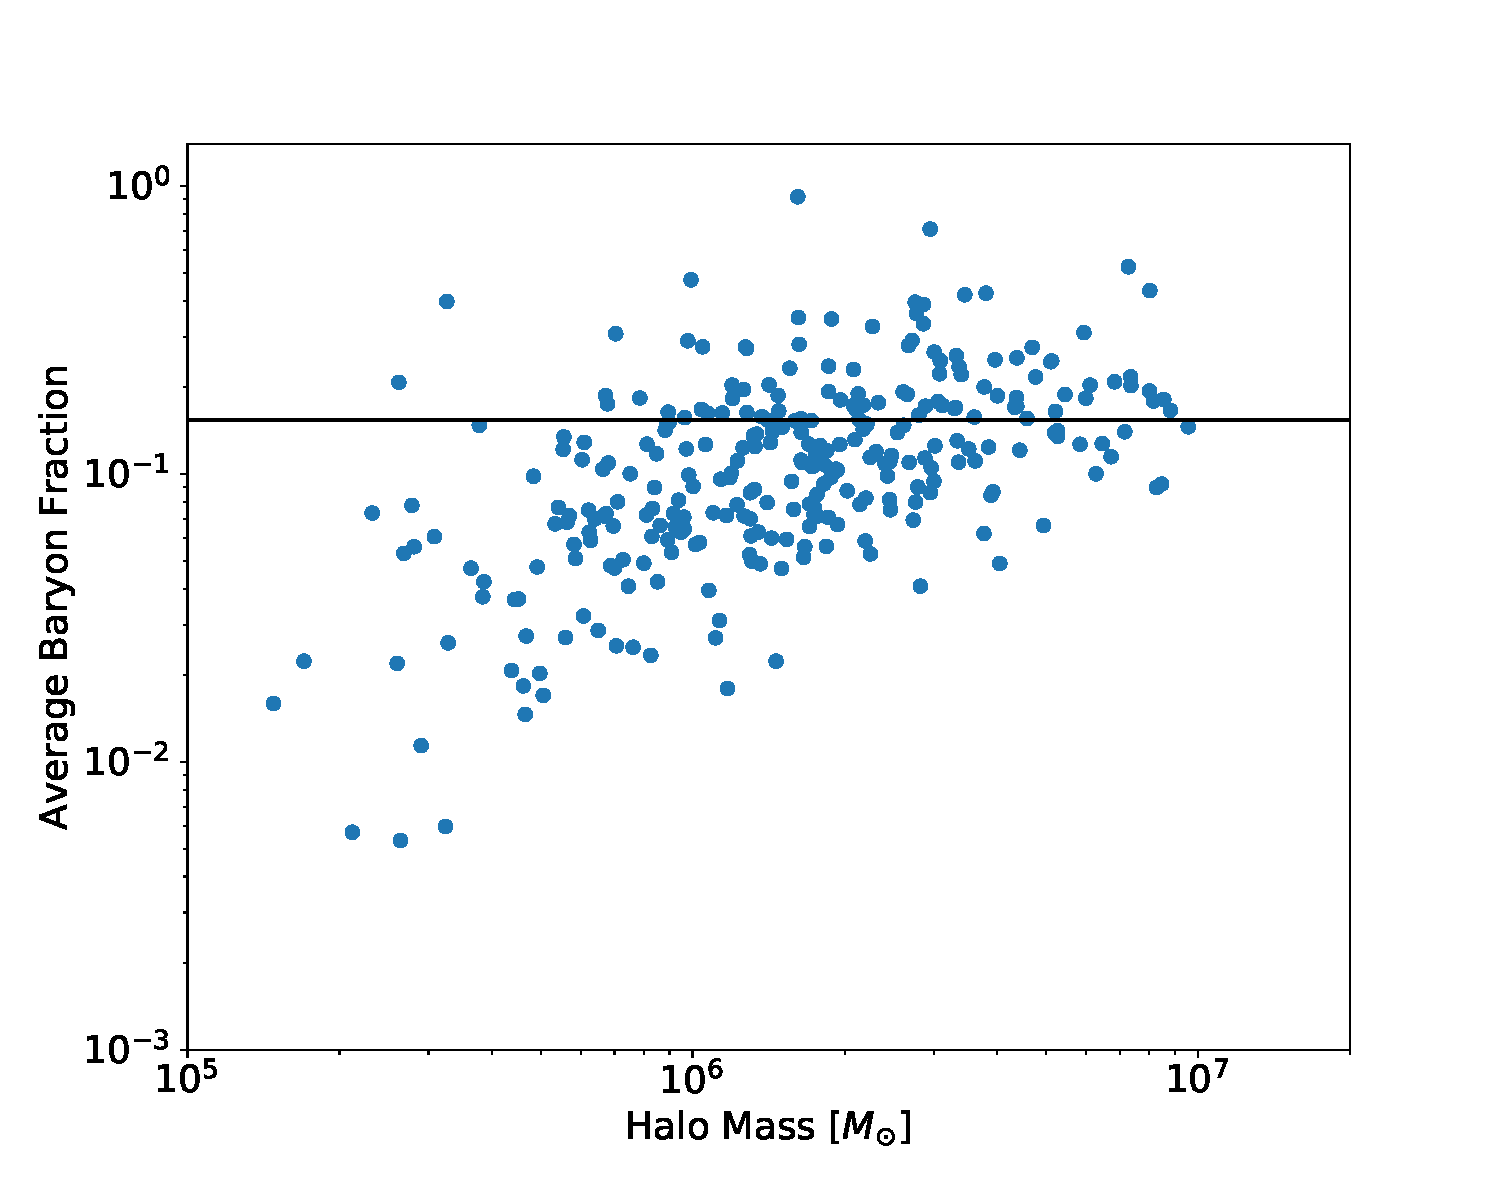
\includegraphics[keepaspectratio=true, scale=0.4]{images/avg_baryon_fraction.pdf}
  \caption{\label{fig:avg_baryon_fraction} Average baryon fraction within each halo versus the corresponding halo mass. The solid line indicates the cosmic baryon fraction of 0.154.}
\end{figure}

\begin{referee}
Minor comments:

E -- The authors should state at one point in the paper for which properties they use comoving or physical units.
\end{referee}
We have clarified this point at the end of the second paragraph in the Simulation Setup section.

\begin{referee}
Introduction:

F -- The authors write that Pop III star formation is generally more massive. While a fraction of the community agrees with that, there is manifoldly cited work that finds low-mass Pop III progenitors, and the authors should not let that unmentioned, but also cite eg Stacy+16, Greif+11 and Clark+11.
\end{referee}

This is a good point about low-mass Pop III stars, and we have included these references in the introduction.

\begin{referee}
G -- The authors name a few processes for suppressing Pop III star formation. For completeness, they should also mention eg X-ray heating (citing eg Jeon+14).
\end{referee}

We have mentioned X-ray heating in the introduction and cited Jeon+14.

\begin{referee}
H -- The authors cite the well-known study from Machacek+01. However, a more recent result would be from the study by Visbal+14, giving a lower mass limit. Since the authors find a lower mass limit than Machacek+01, it would be interesting to see how this compares to the lower mass limit from the more modern paper.
\end{referee}
We have included the $M_{\rm crit}$ function that Visbal+14 use in their study (their Equation 4) for a redshift of 20 as a solid purple line in Figure 10. It appears the Visbal+14 find similar masses as Machacek+01, and when comparing the Machacek+01 for our LWBG and the relation from Visbal+14 at z=20, Visbal+14 find higher halo masses overall.

\begin{referee}
Methods:

I -- In Wise+12, three different environment regions are picked. Please provide more description on the rare peak simulation here and discuss why this one is appropriate in this context.
\end{referee}

RP stands for radiation pressure in Wise+12, not rare peak of the Renaissance Simulations (Xu+ 2016). The simulation is the same size as ours, and contains similar physics, including the radiation pressure and soft UV background, which is why we reference it here. The differences are the inclusion of H2 self-shielding and updated cosmological parameters.
 
\begin{referee}
J -- The initialization at z=130 is very late. I am aware that it is impossible to repeat this simulation starting at an earlier redshift, but would advise for future work.
\end{referee}

In hindsight, we agree that we initialized the simulation too late, even with 2nd order Lagrangian perturbation theory.  The maximum baryon overdensity is 1.64$\bar{\rho}_{\rm b}$, and the maximum DM particle displacement is 2.5 $\times$ (cell width).  In future studies, we will start at earlier times when the evolution is solidly in the linear regime.  We thank the referee for pointing this out.

\begin{referee}
K -- Why do the authors pick a non-zero metalicity threshold for Pop III star formation? How many Pop III stars form between Z=0 and Z=5e-6 Z\_sol?
\end{referee}

We chose this metallicity threshold based on the work of Omukai et al. (2005), Schneider et al. (2006), who found that dust cooling was efficient enough above this metallicity to induce low-mass star formation. About 10\% of Pop III stars form with metallicities between zero and $5 \times 10^{-6} Z_\odot$.  Stars only obtain this extremely low (non-zero) metallicity when metal mixing is incomplete.  This usually occurs when a blastwave is mixing into a nearby halo, and the core collapses before it can fully mix.  Because of the randomness of the IMF sampling and errors from numerical diffusion and other solvers, we do not place great emphasis on stars in this metallicity range.  It is unclear what would be the actual stellar metallicity when it reaches main sequence, given our 0.1 proper pc resolution.  We have made a note of this in Section 2.2.1.

\begin{referee}
L -- What is the physical motivation for a density threshold of 1.e6/cc? Is there convergence?
\end{referee}

Our choice was motivated by both previous work and our refinement strategy rather than convergence. Previous work (e.g. O'Shea et al. 2007; Yoshida et al. 2007) and later groups (e.g. Hirano et al. 2015) have shown that the number density is $\sim 10^6 \cubecm$ at our resolution limit of $0.09$ proper pc at $z=10$.  Secondly, we chose this threshold to be similar to the density that would trigger another level of AMR past our maximum level of 12 (dx = 0.09 proper pc at $z=10$).  At these scales, the grid is primarily refined from the Jeans length criterion, which is resolved by at least 8 cells.  Solving for the density in the Jeans length equation, given a typical temperature $T=300$~K with primordial cooling and a Jeans Length of $8 \times \textrm{dx}$, we obtain a number density $n = 5.7 \times 10^4 \cubecm$.  This number density does not exactly match the chosen density criterion because some oversight when setting up the simulation.  In the case where the density SF criterion is larger than $n$, the gas will continue to condense on a faster timescale than its surroundings.  Thus we are confident that this slight mismatch does not affect our results.

We have added the AMR refinement criteria to Section 2.1 and our motivation to this threshold to Section 2.2.1.

\begin{referee}
M -- Similarly, why do the authors chose a H2 fraction of 1.e-3? (Is is a mass fraction or a number fraction?) How many Pop III stars do not form because of this threshold?
\end{referee}

We chose this critical H$_2$ fraction to match with the values found in previous work (e.g. Yoshida et al. 2007; Omukai et al. 2010) at the density threshold of $10^6 \cubecm$.  It is a number fraction.  We have added to Section 2.2.1 to reflect this detail.

In our original formulation (Abel et al. 2007), we implemented this restriction to avoid spurious star particle formation in D-type ionization fronts that can meet all of the other criteria.  But in the presence of an extremely strong Lyman-Werner flux from a nearby ($\sim$1 pc) star, star formation is unlikely to occur in the shell because it is irradiated and not self-gravitating. The last question is an interesting question, but it is difficult to determine because these conditions (high density but low H$_2$ fractions) are short-lived just after star formation.  Thus we cannot give a definite answer to it, but from the original formulation, we would estimate that the number of Pop III stars would increase by a factor of several with multiple cells in the quasi-spherical ionization front triggering star particle formation.  Because of these uncertainties, we have not added any of these details to the manuscript.

\begin{referee}
N -- Do the authors set fixed mass limits to the IMF and if yes, which are they?  If not, which is the highest / lowest mass they find in their random sampling?  And which fraction of the Pop III stars in the simulation end up as type II SNe / BHs / PISN?
\end{referee}
We do set fixed mass limits, between 1 and 300 $M_{\odot}$. We have added this detail in section 2.2.1.  

59, 36, and 5 per cent of Pop III stars become Type II SN, black holes with no SN, and PISNe respectively. This detail has been added in section 2.2.1.

\begin{referee}
O -- One effect than can weaken the shielding is shifting out of the Lyman-Werner resonance lines (see Hartwig+15). I am wondering how much this would affect the study presented here.
\end{referee}

In Hartwig+15, they take into account the Doppler-shifting of spectral lines with an improved calculation of the column densities, but use the same shielding factor as we do. They find that shielding is generally less efficient at higher temperatures. In our work, because our halos are less massive, the temperatures are typically $10^{3}$ K, which looking at their Figure 5, lies close to the 1:1 line. The shielding factor as calculated in our work will therefore not vary significantly compared to the full treatment of the column density, so we do not expect this to be a problem. 

A brief desription of this has been added to the \hh{} Self-Shielding section. 

\begin{referee}
P -- In Figure 1, please mention in the caption or at the top / bottom of the left axis that a shielding factor of 1 corresponds to no shielding and a shielding factor of 0 corresponds to high shielding, as these nomenclatures are not immediately understandable for the reader.
\end{referee}
This is a tricky detail, and has been added to the caption of Figure 1.

\begin{referee}
Q -- The analytic calculation of the shielding factor is a nice property of the paper. However, assuming a constant H2 fraction seems not appropriate. Please repeat this exercise for a more realistic halo profile, which could be found in the simulations or in the literature, eg by Machacek+01 themselves.
\end{referee}
This is a good point, and the plot has been adjusted accordingly. The halo profiles from O'Shea and Norman 2007 are now being used as the \hh{} fraction as a function of radius. The plot now shows that the shielding factor increases as a function of mass, since at larger radii, there is less \hh{}, resulting in a less effective \hh{} shield. The overall take away of the plot has not changed. 

\begin{referee}
Results:

R -- Figure 2 is quite empty, it would be useful to include the halo mass function of the earliest Pop III formation redshift with its analytic prediction. In addition, the authors could provide a line or an arrow to show their halo mass resolution limit.
\end{referee}
We have added a vertical line at $10^5 M_{\odot}$ to show our halo mass resolution limit. This detail has also been added to the caption.

At the time of the first star formation, our simulation only marginally resolves the smallest main halos, there is only a total of 6 halos above our resolution limit of $10^{5} M_{\odot}$. Because of this, there are not enough halos to accurately represent the HMF at that time, which is why we have not added that to Figure 2. We have added this detail to the first paragraph of the Results section. 

\begin{referee}
S -- Figure 3 looks very nice. It would be helpful if an additional line that only 
provides the global LWBG (in units of J21) was included.
\end{referee}
Thank you for your comment. The global LWBG has been added as a red dashed line. More detail about the LW background (solid red line) has also been added.

\begin{referee}
T -- The authors find no correlation between the host halo mass and the Lyman-Werner background intensity. However, they only look at the LWBG flux at the time of Pop III formation - is there maybe a correlation between the time integrated LW flux?
\end{referee}
While the time integrated LW flux would be interesting to follow, and may provide some further insight to what we are exploring, this would be difficult to calculate. It would require constant tracking of halos through time to calculate the time integrated LW flux. 

\begin{referee}
U -- Figures 7 and 8 show very nice histograms as an additional panel on the right.  I suggest to include a histogram on the spread of the creation time in Figure 9 similar to Figures 7 and 8.
\end{referee}
The side histogram has been added to Figure 9. 

\begin{referee}
Discussion:

V -- The authors give three reasons for the halo mass spread. Can they estimate which of the three processes (BH formation, dynamical heating and temporal LWBG fluctuations) is responsible for the spread by which fraction?
\end{referee}

This is an interesting question, but it is outside the scope of this paper.  It most likely depends on the large-scale environment, halo mass accretion history, and halo star formation history, but how these factors affect each other is unclear.  In practice, it would be difficult to determine the relative importance of dynamical heating and temporal LWBG fluctuations because of the time variations in the heating rate and suppression of H$_2$ cooling.  Because of these reasons, we do not give any estimates in the discussion.

The occurrence of BH formation and no metal enrichment depends on the chosen Pop III IMF, and we have addressed in an earlier answer and noted this fraction in the discussion.

\begin{referee}
W -- One of the most extensive studies on over 1000 minihaloes was performed by Hirano+15, who also include a Lyman-Werner background. Their work should be put in comparison as well.
\end{referee}
This study has been added and cited in the Comparison section.
\textbf{-Should more be added?}

\begin{referee}
X -- In Figure 10, the result from Yoshida+03 is hard to see, maybe use a different symbol / colour.
\end{referee}
We have modified Figure 10 to be more clear. The point from Yoshida+03 is now a pentagon and is outlined in black, and all symbols have had their edges increased for visibility.

\begin{referee}
Y -- Since the authors study star formation in minihaloes, it would be appropriate to also mention Kitayama+04 and Schauer+15 for the Lyman-Werner escape fractions from minihaloes.
\end{referee}
These papers have been added and referenced in the first paragraph of the caveats section. 

\begin{referee}
Z -- The authors mention a few times that streaming velocities are another pathway of suppressing Pop III formation (also in the introduction). While they cite some older work, they however fail to compare to more recent work eg by Hirano+18 or Schauer+19 (who do perform a systematic study not only based on a few, single haloes).
\end{referee}
The Schauer+19 study has been added to the caveat section.

\end{document}
